\section{Konstrukcja prototypu sieci neuronowej}
Po zakończeniu procesu eksploracji danych można przystąpić do konstrukcji sieci
neuronowej odpowiedzialnej za rozpoznawanie ziaren rud miedzi.
Przedstawiony problem wymaga klasyfikacji wieloklasowej wielowymiarowych danych.
Problemy tego typu można rozwiązywać zarówno za pomocą klasycznych algorytmów
uczenia maszynowego jak i~uczenia głębokiego.
Zdecydowano się na wybór sieci neuronowych do klasyfikacji ziaren.
Jest to rozwiązanie najbardziej nowoczesne i~elastyczne.
Zgodnie z~opisem narzędzi programistycznych w~podsekcji
\ref{subsec:software_network},~proces budowania sieci oparto na interfejsie
Keras, z~zapleczem TensorFlow.

\subsection{Dobór struktury sieci}
\label{subsec:nn_build}
Kluczowym czynnikiem decydującym o~architekturze sieci jest posiadany zbiór
danych.
Wejściowy zestaw cech klas jest pięciowymiarowy, do klasyfikacji takich danych
wystarczająca powinna być standardowa sieć neuronowa.
Nie ma potrzeby używania bardziej złożonych sieci rekurencyjnych, czy
konwolucyjnych.

Projektowanie sieci neuronowych wymaga podjęcia szeregu wyborów, wśród nich
można wyróżnić następujące decyzje dotyczące:
\begin{itemize}
    \item ilości warstw sieci,
    \item typu warstw w sieci,
    \item ilości neuronów w~poszczególnych warstwach sieci,
    \item rodzajów funkcji aktywacji w~neuronach poszczególnych warstw sieci.
\end{itemize}
Definiując model należy rozpatrzeć przedstawione cechy budowanej sieci.
Nie istnieje jednoznaczny sposób bezpośredniego określenia najlepszego
klasyfikatora dla danego problemu.
Przy projektowaniu sieci należy kierować się przesłankami teoretycznymi,
doświadczeniem oraz testując i~porównując różne rozwiązania.
Przedstawiona konstrukcja oraz uzasadnienie jej wyboru bazuje na wynikach
walidacji, której mechanizm przedstawiono w~sekcji \ref{sec:nn_validation}.~%
Szczegółowe dane, dotyczące porównań różnych konstrukcji i~parametrów sieci
przedstawiono w~dodatku \ref{ch:nn_comparison_table}.

Konstrukcję klasyfikatora rozpoczęto od wyboru ilości warstw.
W~standardowej konstrukcji każda sieć posiada warstwę wejściową oraz wyjściową,
których parametry są związane odpowiednio z~wektorem cech oraz reprezentacją
klas na wyjściu sieci.
Aby zwiększać efektywność sieci pomiędzy warstwą wejściową oraz wyjściową
umieszcza się zestaw warstw nazywanych \emph{ukrytymi}.
Zazwyczaj posiadają one najwięcej neuronów spośród warstw w~sieci.
Matematycznie dowiedziono, że jedna warstwa ukryta%
\footnote{%
    Przy pewnych obostrzeniach co do doboru funkcji aktywacji.}
wystarcza do aproksymacji dowolnej funkcji nieliniowej
\cite{cybenko_approximations}.
Nie oznacza to jednak, że w~praktyce tak mała sieć wystarczy, aby rozwiązać
dowolny problem uczenia maszynowego.
Dodanie większej ilości warstw ukrytych jest jednym z~najlepszych sposobów na
poprawę działania sieci w~realnych warunkach \cite[str.~273]{geron_ml}.
Biorąc pod uwagę złożoność rozpatrywanego problemu zdecydowano się na strukturę
czterowarstwową (warstwa wejściowa, wyjściowa i~dwie warstwy ukryte).
Jest to rozmiar często spotykany w~sieciach tego typu, późniejsze testy
pokazały, że wybrana liczba warstw daje dobre rezultaty.
Sprawdzono, że zastosowanie jednej warstwy ukrytej powodowało pogorszenie
działania sieci.

Kolejnym krokiem projektowania sieci jest decyzja o~ilości neuronów
w~poszczególnych warstwach.
W przypadku pierwszej i~ostatniej warstwy jest to wartość prosta do określenia.
Zaleca się, aby wejście sieci miało liczbę neuronów równą liczbie elementów
wektora cech, który w~rozpatrywanym przypadku ma długość równą pięć
\cite[str.~272]{geron_ml}.
Ostatnia warstwa powinna mieć tyle neuronów ile wynosi liczba rozpoznawanych
klas, tak by każde wyjście sieci oznaczało prawdopodobieństwo przynależności
próbki do odpowiedniej klasy.
W~analizowanym zbiorze ziaren znajdują się cztery typy rud miedzi i~tyle
neuronów powinno znajdować się w~warstwie wyjściowej sieci.
W~warstwach ukrytych umieszczono większą liczbę neuronów, eksperymentalnie
stwierdzono, że sieć osiąga dobre wyniki dla 256 neuronów w~pierwszej warstwie
ukrytej i~128 w~drugiej.
Zmniejszenie liczby neuronów w~kolejnej warstwie ukrytej jest często spotykanym
zabiegiem.
Obecnie w~skomplikowanych sieciach coraz częściej stosuje się tę samą liczbę
neuronów w~warstwach ukrytych w~celu łatwiejszej parametryzacji modelu
\cite[str.~272]{geron_ml} .
Ponieważ w~rozpatrywanym przypadku liczba warstw jest niewielka, zrezygnowano
z~tej praktyki i~zdecydowano się na podejście polegające na zmniejszeniu liczby
neuronów w~drugiej warstwie ukrytej.

Następnie rozpatrzono dostępne funkcje aktywacji poszczególnych warstw.
Dla warstwy wyjściowej należy wybrać funkcję o~wartościach od zera do jeden.
Jest to uzasadnione faktem, że wyjścia powinny reprezentować prawdopodobieństwo
zaliczenia próbki do danej klasy.
Przy klasyfikacji zazwyczaj stosuje się funkcję softmax, jej wykres
przedstawiono na rysunku \ref{fig:softmax}.%~
\begin{figure}[htb]
    \centering
    \begin{tikzpicture}
        \begin{axis}[title={$ Softmax(z) $}, width=8cm, height=6cm,
                ylabel=$ \sigma(z) $, xlabel=$ z $, xmin=-5, xmax=5]
            \addplot[blue, domain=-5:5, samples=51]
            {exp(x) / sumexp(x, -4, 0)};
        \end{axis}
    \end{tikzpicture}
    \caption{Funkcja aktywacji softmax}
    \label{fig:softmax}
\end{figure}
W~przypadku pozostałych warstw wybór funkcji aktywacji jest mniej oczywisty.
Rozpatrzono trzy rodziny funkcji:
\begin{itemize}
    \item funkcję sigmoid,
    \item funkcje z~grupy jednostek liniowych (ang. \emph{linear unit}):
          \begin{itemize}
              \item ReLU (ang. \emph{Rectified Linear Unit}),
              \item ELU (ang. \emph{Exponential Linear Unit}),
          \end{itemize}
    \item funkcję tangens hiperboliczny.
\end{itemize}
Rozpatrywane funkcje aktywacji przedstawiono na rysunku \ref{fig:activation}.~%
\begin{figure}[htb]
    \hspace*{\fill}
    \begin{subfigure}[t]{0.3\textwidth}
        \centering
        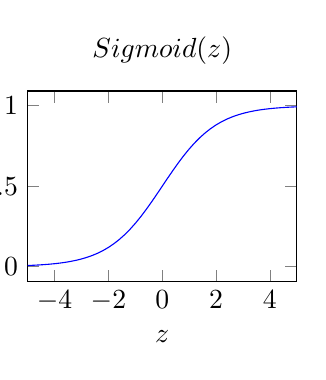
\begin{tikzpicture}[trim axis left]
            \begin{axis}[title={$ Sigmoid(z) $}, width=5cm, height=4cm,
                    ylabel=$ \sigma(z) $, xlabel=$ z $, xmin=-5, xmax=5]
                \addplot[blue, domain=-5:5, samples=51]
                {1 / (1 + e^(-x)};
            \end{axis}
        \end{tikzpicture}
        \caption{Funkcja aktywacji tangens hiperboliczny}
    \end{subfigure}
    \hfill
    \begin{subfigure}[t]{0.3\textwidth}
        \centering
        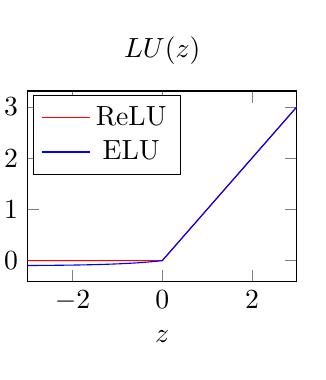
\begin{tikzpicture}[trim axis left]
            \begin{axis}[title={$ LU(z) $}, width=5cm, height=4cm,
                    ylabel=$ \sigma(z) $, xlabel=$ z $, xmin=-3, xmax=3,
                    legend style={at={(0.02, 0.98)}, anchor=north west}]
                \addplot[red, domain=-3:3, samples=31]
                {max(0, x)};
                \addplot[blue, domain=-3:3, samples=31]
                {x < 0 ? 0.1*(e^x - 1) : x};
                \legend{ReLU, ELU}
            \end{axis}
        \end{tikzpicture}
        \caption{Rodzina funkcji aktywacji jednostek liniowych}
    \end{subfigure}
    \hfill
    \begin{subfigure}[t]{0.3\textwidth}
        \centering
        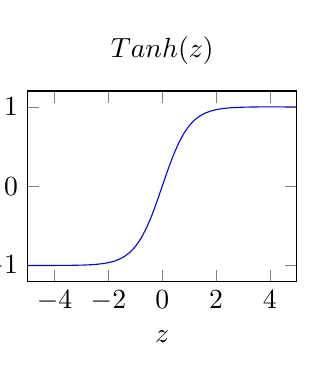
\begin{tikzpicture}[trim axis left]
            \begin{axis}[title={$ Tanh(z) $}, width=5cm, height=4cm,
                    ylabel=$ \sigma(z) $, xlabel=$ z $, xmin=-5, xmax=5]
                \addplot[blue, domain=-5:5, samples=51]
                {tanh(x)};
            \end{axis}
        \end{tikzpicture}
        \caption{Funkcja aktywacji tangens hiperboliczny}
    \end{subfigure}
    \hspace*{\fill}
    \caption{Funkcje aktywacji rozpatrywane do użycia w~warstwach
        ukrytych}
    \label{fig:activation}
\end{figure}
Funkcja sigmoid jest często stosowaną, klasyczną funkcją aktywacji.
Jej wadą jest jednak zanikanie wartości pochodnej.
Obecnie częściej stosowane są funkcję z~rodziny jednostek liniowych,
szczególnie z wyciekiem, czyli małymi wartościami dla ujemnych argumentów.
Przetestowano również funkcję tangens hiperboliczny, która ma kształt
podobny do funkcji sigmoid.
Mimo, że obecnie funkcje jednostek liniowych są najbardziej popularne
w~rozpatrywanym przypadku sieć osiągała najlepsze wyniki dla funkcji tangens.

Opisany model sieci neuronowej należy zdefiniować za pomocą interfejsu Keras.
Do inicjalizacji sieci o~standardowej liniowej strukturze służy funkcja
\mintinline{python}{Sequential()}, która może przyjąć listę warstw w~sieci.
Funkcja \mintinline{python}{Dense()} tworzy warstwę łącząca każdy neuron
z~każdym wyjściem poprzedniej warstwy.
Jej parametry definiują liczbę neuronów w~warstwie oraz ich funkcję aktywacji.
Funkcję języka Python implementują opisywaną sieć, za pomocą przedstawionych
elementów biblioteki Keras, przedstawiono na listingu \ref{lst:model}.
\begin{listing}[htb]
\begin{minted}{python}
def default_grain_classifier_model():
    '''
    Get default uncompiled model for grain classifcation,
    based on 5 step cooling process using number of blobs.
    '''
    model = keras.Sequential([
        keras.layers.Dense(5, activation='tanh'),
        keras.layers.Dense(256, activation='tanh'),
        keras.layers.Dense(128, activation='tanh'),
        keras.layers.Dense(4, activation='softmax')
    ])
    return model
\end{minted}
\caption{Funkcja języka Python definiująca model sieci neuronowej}
\label{lst:model}
\end{listing}

\subsection{Trening sieci neuronowej}
\label{subsec:nn_train}
Kolejnym krokiem w~budowie klasyfikatora ziaren jest trening sieci neuronowej.
Jest to proces. w~którym wagi neuronów są dopasowywane do zbioru uczącego.
Rozpatrywany problem jest typu uczenia nadzorowanego.
Przygotowane dane mają znane etykiety klas, to znaczy są odgórnie przypisane
do danego typu.
Narzucone etykiety nazywane są \emph{wiedzą ekspercką}, ich prawdziwość jest
pewna.
Etykiety przypisane przez klasyfikator będą oceniane przez porównanie
z~etykietami eksperckimi.
Trening polega na zbliżaniu wyników działania sieci do etykiet zbioru uczącego.

Przed rozpoczęciem uczenia sieci należy podzielić dostępne dane na zbiór
treningowy oraz~testowy.
W~skład zbioru testowego nie powinny wchodzić dane uczące.
Ocena zdolności sieci do generalizacji problemu może bazować tylko na danych,
które nie brały udziału w~jej treningu.
Aby ułatwić podział Biblioteka Scikit-learn udostępnia funkcję
\mintinline{python}{train_test_split()}, która zwraca podane zbiory, podzielone
na części treningowe i~testowe.
Odpowiednie wykorzystanie funkcji wymaga użycia jej parametrów opcjonalnych.
Argument \mintinline{python}{stratify} sprawia, że podzielone zbiory zawierają
takie same proporcje klas.
Taka metoda podziału nazywana jest \emph{losowaniem warstowym}.
Uaktywnienie tej opcji jest szczególnie ważne, ze względu na mały rozmiar
posiadanego zbioru danych.
Gdyby dane dzielić w~pełni przypadkowo istniałoby ryzyko nadmiernej
reprezentacji klasy w~danej grupie oraz jej braku w~innej.
Kolejnym istotnym parametrem jest \mintinline{python}{test_size}, który decyduje
o~rozmiarze zbioru testowego.
Ponieważ w~zbiorze są trzy egzemplarze każdej klasy odpowiednie jest wydzielenie
do testów jednej trzeciej próbek.
Ostatni parametr \mintinline{python}{random_state}, to ziarno generatora
losowego podziału zbiorów.
Aby móc porównywać działanie sieci, pomiędzy wielokrotnymi uruchomieniami
programu, należy wyeliminować z~niego czynniki przypadkowe i~podać funkcji stałe
ziarno, co zapewni powtarzalny podział zbioru.
Oczywiście wydzielenie w~narzucony sposób zbioru testowego, szczególnie
w~przypadku tak małej ilości danych, nie daje obiektywnej oceny modelu.
Jest on jednak wystarczający do budowy i~testowania pierwszego prototypu sieci.
W~sekcji \ref{sec:nn_validation}~przedstawiono konstrukcję i~wyniki działania
bardziej miarodajnego procesu walidacji.

Aby móc przystąpić do treningu należy określić parametry uczenia sieci.
Konfiguracja tego procesu odbywa się przez wywołanie metody kompilacji.
Metoda przyjmuje parametry algorytmu optymalizacji sieci, miary błędu oraz
metryki.
Argument \mintinline{python}{optimizer} przyjmuje  nazwę stosowanego algorytmu
uczenia sieci.
Rozważono dwa popularne metody treningu: sgd (ang. \emph{stochastic gradient
descent)} oraz adam (ang. \emph{adaptive moment estimation}).
Metoda sgd jest najbardziej popularnym i~podstawowym sposobem uczenia, jednak
algorytm adam, jest rozwiązaniem nowszym, i~bardziej wydajnym.
Jedną z~zalet drugiego algorytmu jest adaptacyjne obliczanie współczynnika
uczenia, przez co strojenie tego parametru nie jest konieczne.
Wadą nowszego rozwiązania jest spadek jakości wyników dla szczególnych zbiorów
danych \cite[str. 299]{geron_ml}.
Porównanie algorytmów w~rozpatrywanym przypadku wskazało, że algorytm adam daje
lepsze rezultaty i~to na jego użycie się zdecydowano.
Parametr \mintinline{python}{loss} przyjmuje nazwę sposobu liczenia błędu
w~sieci.
Przykładem miary błędu używanej w~sieciach neuronowych jest popularny błąd
średniokwadratowy.
Dla problemów klasyfikacji lepszy jest jednak błąd obliczany metodą
\emph{rzadkiej kategoryzacyjnej entropii krzyżowej} (ang. \textit{sparse
categorical crossentropy}).
Jest to złożona metoda wykorzystująca funkcję logarytmiczną.
Metoda kategoryzacyjnej entropii okazała się najlepszą funkcją błędu dla
analizowanego przypadku.
Ostatni parametr metryki to wartość obliczana w~celu oszacowania poprawności
działania sieci.
Wybrano standardową metrykę dokładności sieci, czyli stosunku poprawnie
zakwalifikowanych próbek do wszystkich analizowanych.

Ostatnim etapem uczenia jest realizacja treningu sieci, dokonywana za pomocą
metody \mintinline{python}{model.fit()}.
Metoda przyjmuje argumenty zbioru treningowego wraz z~zestawem etykiet oraz
liczbę epok treningu, zwraca obiekt zawierający przebieg uczenia sieci.
Na rysunku \ref{fig:training_history}~przedstawiono dokładność i~błąd
w~kolejnych epokach treningu.
Na ich podstawie określono, że odpowiednia liczba epok wynosi 300.
\begin{figure}[htb]
    \hspace*{\fill}
    \begin{subfigure}[t]{0.3\textwidth}
        \centering
        \input{figures/neural_network_trainig_all}
        \caption{Przebieg treningu sieci dla metody zliczania wszystkich
            ziaren}
    \end{subfigure}
    \hfill
    \begin{subfigure}[t]{0.3\textwidth}
        \centering
        \input{figures/neural_network_trainig_remaining}
        \caption{Przebieg treningu sieci dla metody zliczania śledzonych
            ziaren}
    \end{subfigure}
    \hfill
    \begin{subfigure}[t]{0.3\textwidth}
        \centering
        \input{figures/neural_network_trainig_ratio}
        \caption{Przebieg treningu sieci dla metody zliczania stosunku
            śledzonych ziaren}
    \end{subfigure}
    \hspace*{\fill}
    \caption{Przebieg treningu sieci dla różnych metod zliczania ziaren}
    \label{fig:training_history}
\end{figure}
Opisany plan treningu sieci realizuje kod przedstawiony na listingu
\ref{lst:nn_training}.
\begin{listing}[htb]
\begin{minted}{python}
def classification_demo(X, y):
    '''
    Demo grain classification on given data.
    Train and test default model.
    '''
    X = np.array(X)
    y = np.array(y)

    X_train, X_test, y_train, y_test = train_test_split(
        X, y, stratify=y, test_size=0.33, random_state=1)

    model = default_grain_classifier_model()
    model.compile(
        optimizer='adam',
        loss='sparse_categorical_crossentropy',
        metrics=['accuracy'])
    history = model.fit(X_train, y_train, epochs=300, verbose=0)
\end{minted}
\caption{Kod treningu sieci neuronowej klasyfikującej ziarna miedzi}
\label{lst:nn_training}
\end{listing}

Działanie sieci można sprawdzić na zbiorze testowym.
Należy mieć na uwadze, że przy małej ilości danych i~przedstawionym podziale na
zbiory treningowy oraz testowy nie będzie to test miarodajny.
Jest on jednak akceptowalny przy pierwszych testach sieci podczas jej
konstrukcji.
Wyniki działania sieci przedstawia tabela \ref{tab:nn_test}.~%
Przedstawione wartości błędu oraz dokładności potwierdzają przypuszczenia na
temat użyteczności różnych metod zliczania detali, które przedstawiono
w~podsekcji~\ref{subsec:data_vis}.

\begin{table}[htb]
    \centering
    \begin{tabular}{c|C{2cm}|C{2cm}}
        \toprule
        \multirow{2}{*}{Metoda zliczania detali} &
        \multicolumn{2}{c}{Wskaźnik} \\
                                   & Błąd & Dokładność \\
        \midrule
        Wszystkie detale           & 1,45 & 0,25       \\
        Śledzone detale            & 7,50 & 0,5        \\
        Stosunek śledzonych detali & 0,63 & 0,75       \\
        \bottomrule
    \end{tabular}
    \caption{Wskaźniki oceny działania sieci na zbiorze testowym}
    \label{tab:nn_test}
\end{table}

\section{Walidacja i~ocena działania sieci}
\label{sec:nn_validation}
Po stworzeniu prototypu klasyfkiatora przedstawionego w~rozdziale
\ref{subsec:nn_build}~należy przeprowadzić walidację zbudowanej sieci
neuronowej.
Najpopularniejszą metodą miarodajnej walidacji sieci jest \emph{k-krotny
sprawdzian krzyżowy} (ang. \textit{k-fold cross-validation}).
Metoda ta polega na podziale dostępnych danych na k części, i~kolejnym
wydzielaniu jednej z~części danych jako zbioru testowego.
Walidacje powtarza się k-krotnie, tak by każda część była wykorzystana jako dane
testowe.
Na końcu testu wyniki są uśrednianie.
Dzięki temu sprawdzian krzyżowy daje dobry pogląd na ogólną zdolność sieci do
generalizacji rozwiązywanego problemu.

Często po procesie walidacji dokonuje się testu sieci przy użyciu osobnego
zestawu danych.
Niestety posiadany zbiór jest zbyt mały, aby wydzielić z niego osobny zestaw
testowy.
Z~tego powodu zdecydowano się oceniać sieć jedynie na podstawie metody
sprawdzianu krzyżowego.

Biblioteka Keras nie posiada wbudowanych funkcji zaawansowanych technik
walidacji, dlatego należy przygotować je samodzielnie.
W~tym celu użyto biblioteki Scikit-learn, która oferuje funkcje podziału zbiorów
danych.
Jedną z~nich jest funkcja zwracająca iterowalny zestaw k-krotnych podziałów
zbioru danych.
Jak przedstawiono w~sekcji \ref{subsec:nn_train},~ze względu na mały rozmiar
zbioru danych, przy podziale należy zastosować losowanie warstwowe.
Na listingu \ref{lst:nn_crossval}~przedstawiono funkcję pozwalającą na walidację
modelu klasyfikatora biblioteki Keras z~użyciem sprawdzianu krzyżowego.
Funkcja przyjmuje argumenty w~postaci skompilowanego modelu sieci oraz zbioru
danych i~etykiet.
Zwracana jest macierz, w~której rzędy oznaczają wyniki testów dla kolejnych
podziałów zbioru danych.
\begin{listing}[htb]
\begin{minted}{python}
def network_cross_validation(model, X, y, n_splits):
    '''Compute cross validation fold scores for given keras model.'''
    eval_scores = []

    folds = StratifiedKFold(n_splits=n_splits).split(X, y)
    for train_index, test_index in folds:
        x_train, x_test = X[train_index], X[test_index]
        y_train, y_test = y[train_index], y[test_index]

        model.fit(x_train, y_train, epochs=300, verbose=0)
        eval_scores.append(model.evaluate(x_test, y_test, verbose=0))
    return eval_scores
\end{minted}
\caption{Funkcja języka Python definiująca model sieci neuronowej}
\label{lst:nn_crossval}
\end{listing}
Sposób wykorzystania zbudowanej funkcji walidacji modelu przedstawia listing
\ref{lst:nn_validation}.~%
Na końcu procesu oceny sieci wyniki kolejnych kroków sprawdzianu krzyżowego
należy uśrednić.
Efekty walidacji dla trzech sposobów zliczania detali na obrazach przedstawia
tabela \ref{tab:nn_crossval}.

Zgodnie z~wcześniejszymi przewidywaniami, metoda zliczania stosunku śledzonych
detali do ich pierwotnej liczby okazała się dawać najlepsze rezultaty.
Dokładność na poziomie 91\%~jest wystarczająca do uznania sieci za dobry
klasyfikator.
Pozostałe metody zliczania okazały się mniej precyzyjne, co wskazuje że należy
je odrzucić.

Przedstawiony mechanizm walidacji wykorzystano do dostrojenia parametrów sieci
opisywanych w~podeskcji \ref{subsec:nn_build}.~%
Uzasadnienie doboru przedstawionej w~toku pracy struktury sieci wynika z~prób
maksymalizacji dokładności oblicznej przy pomocy sprawdzianu krzyżowego.
W~czasie prototypowania sieci dokonano liczbych porównań, aby znaleźć najlepszą
strukturę.
Szczegółowe zestaweienie rozpatrywanych konfiguracji i~wartości parametrów
załączono w~dodatku \ref{ch:nn_comparison_table}.

\begin{listing}[htb]
\begin{minted}{python}
def cross_val_demo(X, y):
    '''
    Demo cross validation of default grain classifier
    on given data.
    '''
    X = np.array(X)
    y = np.array(y)

    model = default_grain_classifier_model()
    model.compile(
        optimizer='adam',
        loss='sparse_categorical_crossentropy',
        metrics=['accuracy'])

    scores = network_cross_validation(model, X, y, 3)

    print('Folds scores: (loss, acc)\n', scores)
    scores = np.array(scores)
    print('Cross validation mean score (loss, acc):\n',
            scores.mean(axis=0), '\n')
\end{minted}
\caption{Wykorzystanie funkcji sprawdzianu krzyżowego do oceny działania sieci}
\label{lst:nn_validation}
\end{listing}

\begin{table}[htb]
    \centering
    \begin{tabular}{c|C{2cm}|C{2cm}}
        \toprule
        \multirow{2}{*}{Metoda zliczania detali} &
        \multicolumn{2}{c}{Wskaźnik} \\
                                   & Błąd & Dokładność \\
        \midrule
        Wszystkie detale           & 6,59 & 0,41       \\
        Śledzone detale            & 3,99 & 0,50       \\
        Stosunek śledzonych detali & 1,37 & 0,91       \\
        \bottomrule
    \end{tabular}
    \caption{Wskaźniki oceny działania sieci uzyskane metodą sprawdzianu
        krzyżowego}
    \label{tab:nn_crossval}
\end{table}

Dodatkowo opracowano kod generujący \emph{macierz pomyłek} (ang.
\textit{confusion matrix}).
Jest to tablica porównująca wiedzę eksperta z~wynikami klasyfikacji na zbiorze
testowym.
Wiersze macierzy oznaczają poprawną klasyfikację kolejnych próbek, zgodnie
z~etykietami eksperckimi.
Kolumny tabeli to typy klasyfikatora.
Przekątna tabeli zawiera informacje o~elementach poprawnie sklasyfikowanych,
etykiety klasyfikatora są zgodne z~danymi eksperckimi.
Komórki spoza przekątnej oznaczają błędną klasyfikację.
Obserwacja macierzy pozwala zaobserwować, które typy ziaren są ze sobą mylone
w~trakcie klasyfikacji.

Ze względu na małą ilość posiadanych danych macierz pomyłek opracowano
na podstawie mechanizmu sprawdzianu krzyżowego.
Na każdym jego etapie budowano macierz pomyłek, a~ostatecznie tablicę
uśredniono.
Ułamki dziesiętne w~tabeli reprezentują jaka część próbek danej klasy została
sklasyfikowana w~dany sposób.
Funkcję generującą uśrednioną macierz pomyłek przedstawia listing
\ref{lst:mean_confusion_matrix}.
\begin{listing}[htb]
\begin{minted}{python}
def mean_confusion_matrix(model, X, y, n_splits):
    '''
    Compute mean confusion matrix using cross validation
    with n splits.
    '''
    conf_matrix = np.zeros((4, 4))

    folds = StratifiedKFold(n_splits=n_splits).split(X, y)
    for train_index, test_index in folds:
        x_train, x_test = X[train_index], X[test_index]
        y_train, y_test = y[train_index], y[test_index]

        model.fit(x_train, y_train, epochs=300, verbose=0)
        y_pred = model.predict_classes(x_test)

        for test, pred in zip(y_test, y_pred):
            conf_matrix[test][pred] = conf_matrix[test][pred] + 1

    return conf_matrix / n_splits
\end{minted}
\caption{Funkcja języka Python generująca uśrednioną macierz pomyłek}
\label{lst:mean_confusion_matrix}
\end{listing}

Zdecydowano się wygenerować macierz pomyłek dla najlepszego sposobu
klasyfikacji, bazującego na określaniu stosunku pozostałych detali do ich liczby
na początku procesu stygnięcia.
Wyniki zestawiono w~tabeli \ref{tab:confusion_matrix}.~%
Zgodnie z~wynikami sprawdzianu krzyżowego, większość elementów tablicy znajduje
się na jej przekątnej.
To znaczy, że wszystkie próbki klas E5R, E11R oraz E16R są poprawnie
klasyfikowane.
Widoczna jest pomyłka sieci polegająca na niewłaściwej klasyfikacji próbki klasy
E6R jako E16R.

\begin{table}[htb]
    \centering
    \begin{tabular}{cccccc}
        & & \multicolumn{4}{c}{Wiedza klasyfikatora} \\
        \cmidrule[1pt]{2-6}
        & \multicolumn{1}{c|}{klasa} & E5R  & E6R  & E11R & E16R \\
        \cmidrule{2-6}
        \multirow{4}{*}{\rotatebox[origin=c]{90}{\parbox{2cm}
        {\centering Wiedza eksperta}}} 
            & \multicolumn{1}{c|}{E5R}   & 1,00 & 0,00 & 0,00 & 0,00 \\
            & \multicolumn{1}{c|}{E6R}   & 0,00 & 0,67 & 0,00 & 0,33 \\
            & \multicolumn{1}{c|}{E11R}  & 0,00 & 0,00 & 1,00 & 0,00 \\
            & \multicolumn{1}{c|}{E16R}  & 0,00 & 0,00 & 0,00 & 1,00 \\
        \cmidrule[1pt]{2-6}
    \end{tabular}
    \caption{Tabela pomyłek najlepszego klasyfikatora}
    \label{tab:confusion_matrix}
\end{table}
